% === Begin Label Data ===
% ID: 442
% 难度星级: 
% 标签: 
% 备注: 
% 组卷引用次数: 0
% === End  Label Data ===

\begin{problem}{2017}{G}{新课标I卷}{16}{立体几何}
如图，圆形纸片的圆心为 $ O $，半径为 $ 5\,\text{cm} $，该纸片上的等边三角形 $ ABC $ 的中心为 $ O $，$ D,E,F $ 为圆 $ O $ 上的点。$ \triangle DBC $、$ \triangle ECA $、$ \triangle FAB $ 分别是以 $ BC $、$ CA $、$ AB $ 为底边的等腰三角形。沿虚线剪开后，分别以 $ BC $、$ CA $、$ AB $ 为折痕折起 $ \triangle DBC $、$ \triangle ECA $、$ \triangle FAB $，使得 $ D,E,F $ 重合，得到三棱锥。当 $ \triangle ABC $ 的边长变化时，所得三棱锥体积（单位：$ \text{cm}^3 $）的最大值为\underline{\hspace{4em}}.
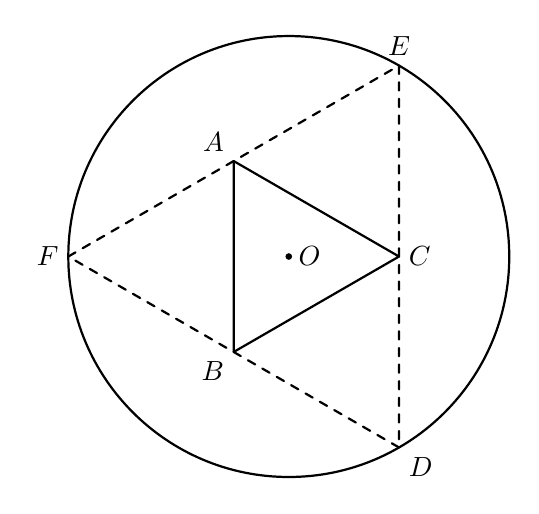
\begin{tikzpicture}[scale=1.0, line cap=round, line join=round]
\usetikzlibrary{calc}
\def\R{2.8}

\coordinate (O) at (0,0);
\coordinate (E) at (60:\R);
\coordinate (D) at (-60:\R);
\coordinate (F) at (180:\R);

\coordinate (A) at ($(F)!0.5!(E)$);
\coordinate (B) at ($(F)!0.5!(D)$);
\coordinate (C) at ($(E)!0.5!(D)$);

\draw[thick] (O) circle (\R);

\draw[dashed, thick] (F)--(E)--(D)--cycle;

\draw[thick] (A)--(B)--(C)--cycle;

\fill (O) circle (1.2pt);
\node[right] at (O) {$O$};

\node[above] at (E) {$E$};
\node[below right] at (D) {$D$};
\node[left] at (F) {$F$};

\node[above left] at (A) {$A$};
\node[below left] at (B) {$B$};
\node[right] at (C) {$C$};
\end{tikzpicture}
\end{problem}

\begin{answer}

\end{answer}

\begin{solutions}

\end{solutions}